% !TeX encoding = UTF-8
% !TeX program = xelatex
% ============================================================================
% NSL-KDD 网络入侵检测系统 —— 课程论文 (CJC 模板)
% 编译: latexmk -xelatex cjc-main.tex  或  make cjc
% ============================================================================

\documentclass{cjc}

\usepackage{booktabs}
\usepackage{algorithm}
\usepackage{algorithmic}
\usepackage{siunitx}
\usepackage{graphicx}
\usepackage{float}

\classsetup{
  title        = {基于NSL-KDD数据集的网络入侵检测研究——传统机器学习与深度学习方法对比},
  title*       = {Network Intrusion Detection Based on NSL-KDD Dataset: A Comparative Study of Traditional Machine Learning and Deep Learning Methods},
  authors      = {
    author1 = {
      name         = {刘卫},
      name*        = {LIU Wei},
      affiliations = {aff1},
      biography    = {},
      biography*   = {},
      email        = {},
    },
    author2 = {
      name         = {查恩鹏},
      name*        = {ZHA En-Peng},
      affiliations = {aff1},
      biography    = {},
      biography*   = {},
      email        = {},
    },
    author3 = {
      name         = {陈安旭},
      name*        = {CHEN An-Xu},
      affiliations = {aff1},
      biography    = {},
      biography*   = {},
      email        = {},
    },
  },
  affiliations = {
    aff1 = {
      name  = {青海大学\ 计算机技术与应用学院, 青海\ 西宁\ 810016},
      name* = {School of Computer Technology and Applications, Qinghai University, Xining 810016, China},
    },
  },
  abstract     = {
    本文基于NSL-KDD数据集（训练集125,973条，测试集22,544条），构建了一个完整的网络入侵检测系统（IDS）。
    通过特征工程将原始41维特征降维至20维关键特征，对比评估了10种模型（包括决策树、随机森林等传统方法，
    以及MLP、CNN、LSTM等深度学习方法）在二分类和多分类任务上的性能。
    实验结果表明，在验证集上神经网络方法显著优于传统机器学习方法，MLP的AUC达到0.999；
    但在统一测试集上两者性能差距缩小——MLP的F1值约为0.72，决策树约为0.76。
    多分类任务受测试集15种训练未见攻击和小样本类别的双重制约，全量准确率上限约10\%。
    本文系统分析了各模型的适用场景与局限性，为NSL-KDD入侵检测任务提供了全面的实验基准和方法论参考。
  },
  abstract*    = {
    This paper presents a comprehensive network intrusion detection system (IDS) based on the NSL-KDD dataset
    (125,973 training samples, 22,544 test samples). Through feature engineering, the original 41-dimensional
    feature space is reduced to 20 key features. A total of 10 models are systematically compared, including
    traditional machine learning methods (Decision Tree, Random Forest) and deep learning methods (MLP, CNN, LSTM),
    evaluated on both binary classification and multi-class attack recognition tasks. Experimental results show
    that deep learning methods significantly outperform traditional methods on the validation set, with MLP achieving
    an AUC of 0.999. However, on the unified test set, the performance gap narrows considerably—MLP achieves an F1
    score of approximately 0.72, while Decision Tree reaches 0.76. Multi-class classification is constrained by
    15 unseen attack types in the test set and extreme class imbalance, with full accuracy capped at approximately
    10\%. This paper provides a comprehensive experimental benchmark and methodological reference for NSL-KDD
    intrusion detection research.
  },
  keywords     = {网络入侵检测, NSL-KDD, 机器学习, 深度学习, 决策树, 随机森林, 对比分析},
  keywords*    = {network intrusion detection, NSL-KDD, machine learning, deep learning, decision tree, random forest, comparative analysis},
  clc          = {},
  doi          = {},
}

\newcommand\dif{\mathop{}\!\mathrm{d}}

% Graphics path
\graphicspath{{../outputs/figures/}}

% hyperref always loaded last in preamble
\usepackage{hyperref}

% Course assignment: suppress journal-specific header/footer on first page
\fancypagestyle{title}{%
  \fancyhf{}%
  \renewcommand{\headrulewidth}{0pt}%
}
% Also suppress running header on all pages (keep page number)
\fancypagestyle{plain}{%
  \fancyhf{}%
  \renewcommand{\headrulewidth}{0pt}%
  \fancyfoot[C]{\thepage}%
}
\pagestyle{plain}


\begin{document}

\maketitle

% ============================
% Chapters
% ============================
\section{绪论}

\subsection{研究背景}

随着互联网规模的持续扩大和网络应用的日益复杂，网络安全面临着前所未有的挑战。网络入侵检测系统（Intrusion Detection System, IDS）作为网络安全的核心防御机制之一，承担着识别异常流量、检测潜在攻击的重要职责。传统的入侵检测方法主要依赖基于规则的特征匹配和专家系统，这种方式需要人工维护庞大的规则库，对零日攻击和未知变种缺乏自适应能力，难以应对日益增长的网络威胁。

近年来，机器学习与深度学习技术的快速发展为入侵检测提供了新的解决思路~\cite{sharma2025machine,akuthota2025role}。通过从海量网络流量数据中自动学习行为模式，数据驱动的方法能够有效捕捉传统规则难以描述的复杂特征，显著提升检测的准确率和泛化能力。基于这一背景，本文以经典的NSL-KDD数据集为研究对象，系统比较多种机器学习模型在二分类与多分类入侵检测任务中的性能差异。

\subsection{NSL-KDD数据集}

NSL-KDD数据集是KDD Cup 1999数据集的改进版本，由Tavallaee等人提出~\cite{tavallaee2009}，针对原始KDD-99中存在的大量冗余记录和测试集样本分布不合理等问题进行了优化，是当前入侵检测研究中被广泛采用的基准数据集之一~\cite{rehman2025systematic}。该数据集由训练文件KDDTrain+.txt和测试文件KDDTest+.txt两部分构成，训练集包含125,973条网络连接记录，测试集包含22,544条记录。

每条记录由41个特征属性和1个类别标签组成。根据特征所描述的信息层次，可将其划分为四组：9个TCP连接基本特征，描述连接的基本属性如协议类型、服务类型、连接持续时间等；13个内容特征，刻画连接内部的用户行为模式；9个时间流量特征，反映最近2秒内与当前连接具有相同主机的统计信息；10个主机流量特征，基于100个连接窗口统计目标主机的流量行为。

数据集中的标签包含一种正常类型（normal）和四种大类攻击：拒绝服务攻击（Denial of Service, DoS）、探测攻击（Probe）、远程到本地攻击（Remote to Local, R2L）以及权限提升攻击（User to Root, U2R），共涵盖23种具体攻击类型。值得注意的是，测试集包含约14种在训练集中未出现的新型攻击样本，例如apache2、httptunnel、mailbomb、mscan、named、processtable、saint、sendmail、snmpgetattack、snmpguess、sqlattack、udpstorm、worm、xterm等。这种设计使得数据集能够有效评估模型对未知攻击的泛化能力，也成为多分类任务中准确率难以突破100\%的重要原因。

\subsection{攻击类别分布}

训练集与测试集在样本分布上呈现出明显的差异。二分类层面，训练集中正常样本占比约53.5\%，异常样本占比约46.5\%，分布相对均衡；而测试集中异常样本占比上升至56.9\%，正常样本下降至43.1\%，与真实网络环境中异常流量占比偏高的实际情况更为接近，具体的二分类标签分布如图1所示。

\begin{figure*}[t]
  \centering
  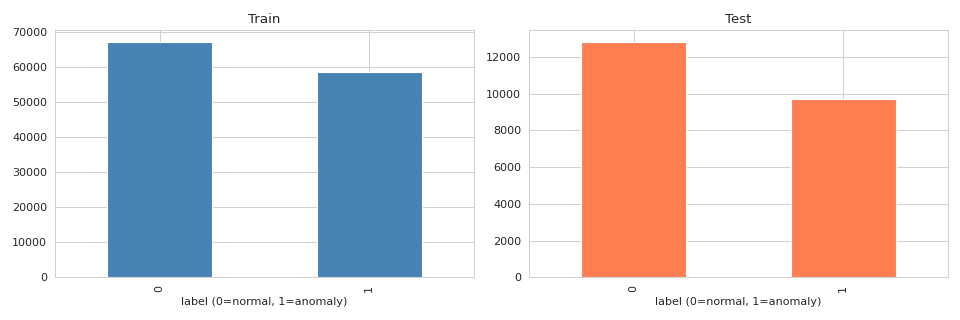
\includegraphics[width=\textwidth]{01_binary_label_distribution.png}
  \caption{训练集与测试集二分类标签分布}
  \label{fig:ch1-01}
\end{figure*}

四类攻击的样本数量差异极为悬殊。训练集中DoS攻击占据主导地位，样本数高达45,927条；Probe攻击次之，为11,656条；而R2L仅有995条，U2R更是仅52条，呈现出严重的长尾分布特征。测试集延续了这种不均衡格局，但各类别间的比例有所变化，大类攻击的整体分布情况如图2所示。

\begin{figure*}[t]
  \centering
  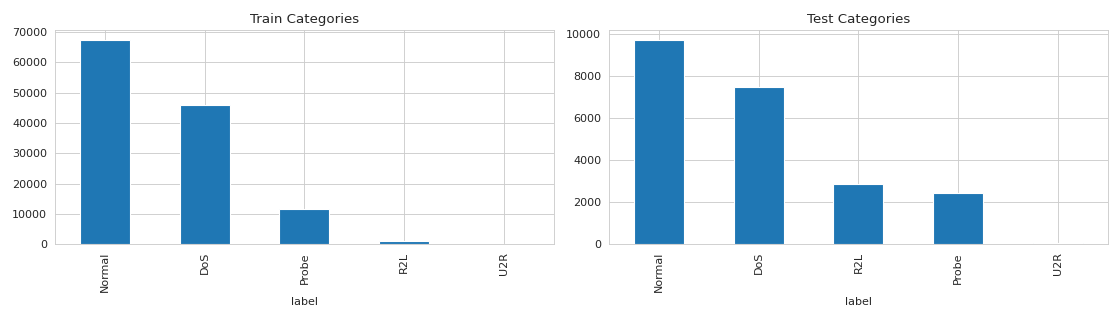
\includegraphics[width=\textwidth]{02_attack_category_distribution.png}
  \caption{训练集与测试集四类攻击大类分布}
  \label{fig:ch1-02}
\end{figure*}

为更细致地展示数据特点，图3给出了训练集与测试集中样本数量排名前15位的具体攻击类型。

\begin{figure*}[t]
  \centering
  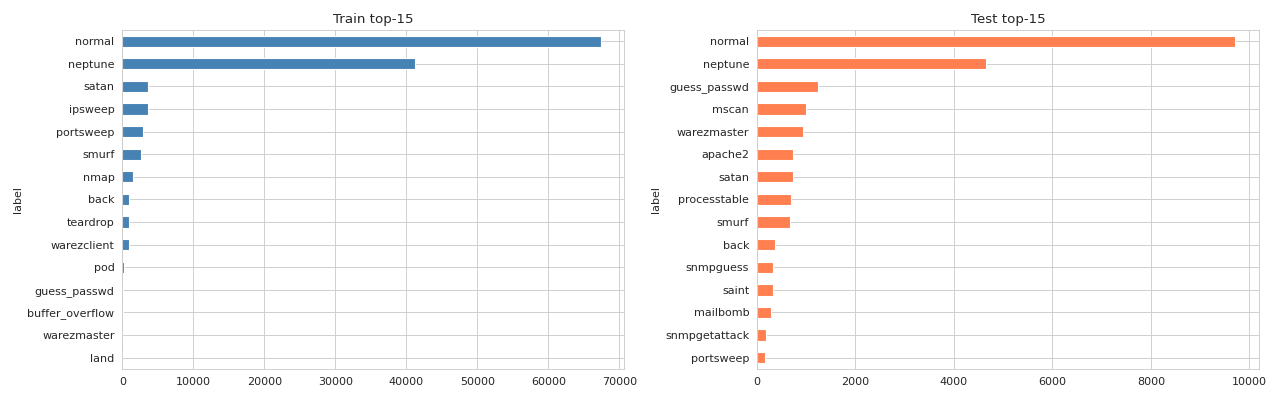
\includegraphics[width=\textwidth]{03_attack_type_top15.png}
  \caption{训练集与测试集中样本数量Top-15攻击类型}
  \label{fig:ch1-03}
\end{figure*}

这种类别不平衡现象，特别是R2L和U2R样本的极度稀缺，是入侵检测建模中需要重点关注的挑战。

\subsection{研究目标与论文结构}

本文的研究目标是基于NSL-KDD数据集，构建并系统比较多种机器学习模型在网络入侵检测任务中的性能表现，重点关注二分类异常检测以及23种攻击类型的细粒度多分类识别能力（在结果分析中按五大攻击类别Normal、DoS、Probe、R2L、U2R进行分组讨论）。同时，深入分析类别不平衡、未知攻击泛化等实际应用中的关键问题，为入侵检测模型的工程落地提供参考依据。

本文共分为五章。第2章将详细介绍数据预处理流程，包括缺失值与异常值处理、类别型特征编码、数值型特征变换以及特征重要性筛选等关键步骤。
\section{数据预处理}

\subsection{数据清洗}

首先对原始NSL-KDD数据集进行质量检查。经逐列扫描确认，41个特征列与1个标签列均不存在缺失值，因此无需进行填充或删除操作。但数据集中附带一列名为difficulty的字段，该字段为Tavallaee等人在构建NSL-KDD时引入的样本难度评分，与网络入侵检测任务本身无关，属于冗余信息，故予以删除。清洗后保留全部125,973条训练记录与22,544条测试记录，特征列从42列缩减为41列（其中38列为数值型，3列为分类型）。清洗后的数值特征整体分布情况如图~\ref{fig:ch2-numeric-dist}所示，三类分类特征的Top-10取值分布如图~\ref{fig:ch2-categorical}所示，可以观察到多数数值特征呈现明显的右偏长尾分布。

\subsection{分类特征编码}

NSL-KDD数据集包含三个字符串类型的分类特征：protocol\_type共3种取值（tcp、udp、icmp），其中tcp占据绝大多数；service共70余种取值，http最为常见；flag共11种取值，SF标志位占比最高。这种长尾分布的分类特征无法直接输入到数值型模型中，需要进行编码转换。

本文采用OneHot编码（OneHotEncoder）策略，将每个分类特征的每个取值转换为独立的二元特征列。具体而言，protocol\_type展开为3列，service展开为70列，flag展开为11列，去除原3个分类列后新增84列，最终特征维度从41维扩展至53维。这种编码方式完整保留了所有类别信息，避免了人为引入序数关系，对树模型与神经网络均友好。

\subsection{异常值处理}

网络流量数据中广泛存在离群点，而入侵检测任务中的离群点往往正是攻击流量的体现。若简单删除异常值所在行，会导致大量稀有攻击样本被错误清除，对检测性能产生负面影响。因此本文采用检测但不删除的策略：使用IQR方法（1.5倍四分位距）识别超出上下边界的取值，再使用clip截断策略将越界值替换为对应的边界值。

受异常值影响最严重的两个特征分别是srv\_diff\_host\_rate（异常率22.5\%）和dst\_host\_same\_src\_port\_rate（异常率19.9\%）。这两个特征本质上反映了扫描类攻击的统计指标，分布本身就具有显著的偏态特征，截断后仍能保留绝大部分判别信息。所有数值特征的相关系数热力图如图~\ref{fig:ch2-correlation}所示，可以观察到内容特征组内部存在较高相关性，而主机流量特征组与时间流量特征组之间也存在若干强相关对。

\subsection{长尾特征变换}

针对src\_bytes、dst\_bytes、count、srv\_count四个流量类特征的严重右偏分布，本文应用log1p变换（即$\log(1+x)$）进行压缩。这四个特征的原始取值跨度可达数个数量级，少数极大值会主导模型的梯度更新方向。log1p变换能够将偏态分布拉近正态，同时对零值保持兼容。变换前后的分布对比见图~\ref{fig:ch2-log1p}，原本集中在零附近且具有长尾的分布在变换后扩展为更接近正态的钟形分布。

\subsection{特征选择}

特征选择分两步执行，以在保留判别信息的同时降低维度、缓解过拟合。

第一步为方差阈值过滤。使用VarianceThreshold方法剔除方差接近零的特征列，主要清除OneHot编码后取值几乎全为零的稀疏列。该步骤将特征数从53维降至32维。

第二步为基于随机森林的特征重要度筛选。在训练集上拟合随机森林模型，按特征重要度从高到低排序，保留Top-20特征。最终特征重要度分布如图~\ref{fig:ch2-importance}所示。Top-5特征分别为：flag\_SF（重要度0.148）、same\_srv\_rate（0.108）、dst\_host\_srv\_count（0.105）、dst\_host\_same\_srv\_rate（0.081）、diff\_srv\_rate（0.076）。从排序可以看出，连接状态标志位以及目标主机的服务统计特征对入侵检测最具判别力，这与已有文献的结论一致。

\subsection{数据划分与持久化}

数据划分遵循NSL-KDD官方方案，训练集使用KDDTrain+.txt，测试集使用KDDTest+.txt，不进行随机重划分，以保证与已有研究结果的可比性。最终训练集形状为$(125973, 20)$，测试集形状为$(22544, 20)$，与原始数据集保持完全一致的样本规模。预处理过程中各阶段的特征维度变化路径如表~\ref{tab:dim-path}所示。

\begin{table}[htbp]
\centering
\caption{预处理各阶段特征维度变化}
\label{tab:dim-path}
\begin{tabular}{lcl}
\toprule
处理阶段 & 维度数 & 说明 \\
\midrule
原始数据 & 41 & 38数值特征 + 3分类特征 \\
OneHot编码 & 53 & 分类特征独热扩展 \\
异常值clip & 53 & 仅截断，维度不变 \\
log1p变换 & 53 & 对4个流量特征应用 \\
方差阈值过滤 & 32 & 移除低方差列 \\
RF Top-20筛选 & 20 & 按重要度排序取前20 \\
\bottomrule
\end{tabular}
\end{table}

处理完成后的数据以pickle格式持久化，保存于\texttt{outputs/processed/}目录下，共生成8个文件，分别对应训练集与测试集的特征矩阵与标签向量的二分类与五分类版本，便于后续模型加载使用。

\begin{figure*}[htbp]
\centering
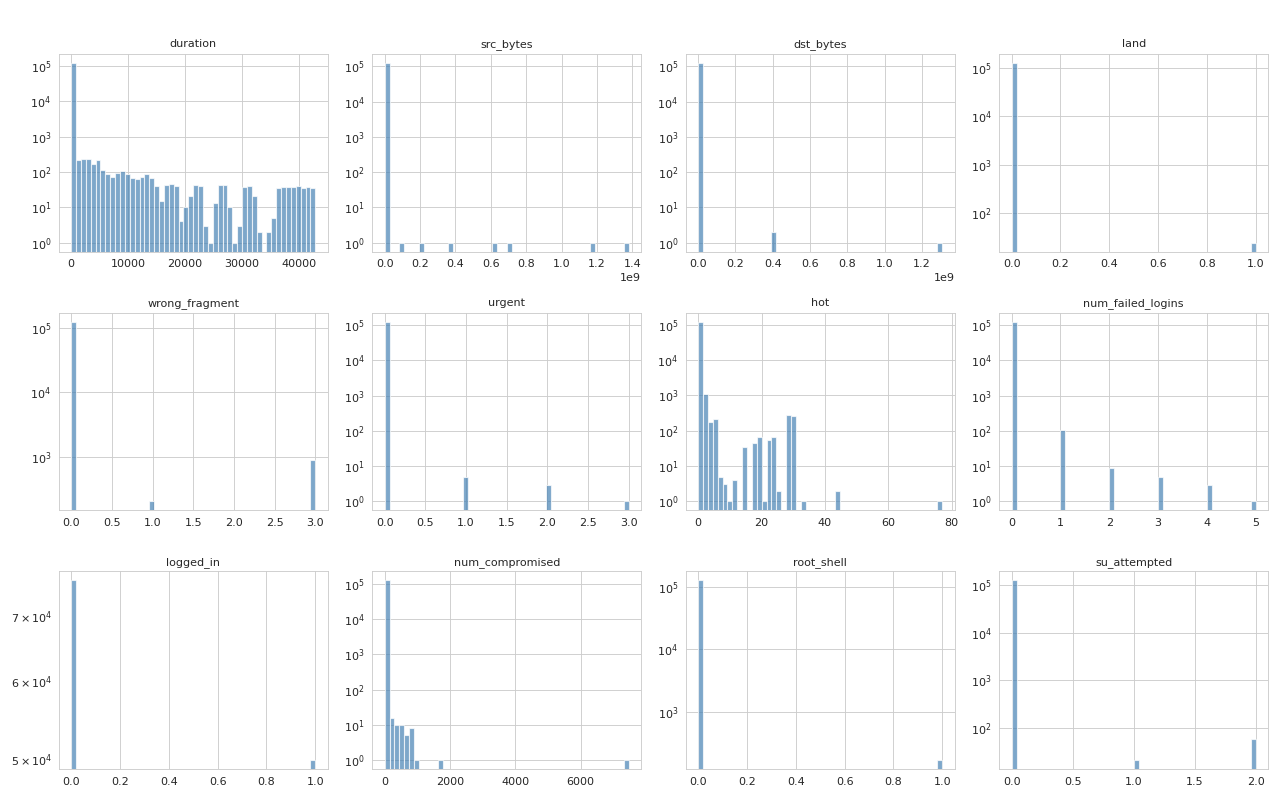
\includegraphics[width=\textwidth]{04_numeric_distributions.png}
\caption{数值特征分布}
\label{fig:ch2-numeric-dist}
\end{figure*}

\begin{figure}[htbp]
\centering
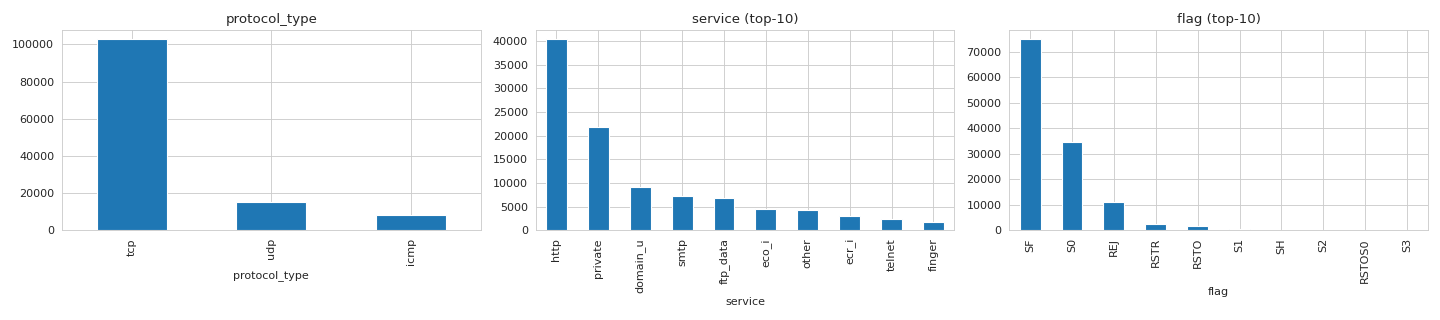
\includegraphics[width=\columnwidth]{05_categorical_top10.png}
\caption{分类特征Top-10分布}
\label{fig:ch2-categorical}
\end{figure}

\begin{figure*}[htbp]
\centering
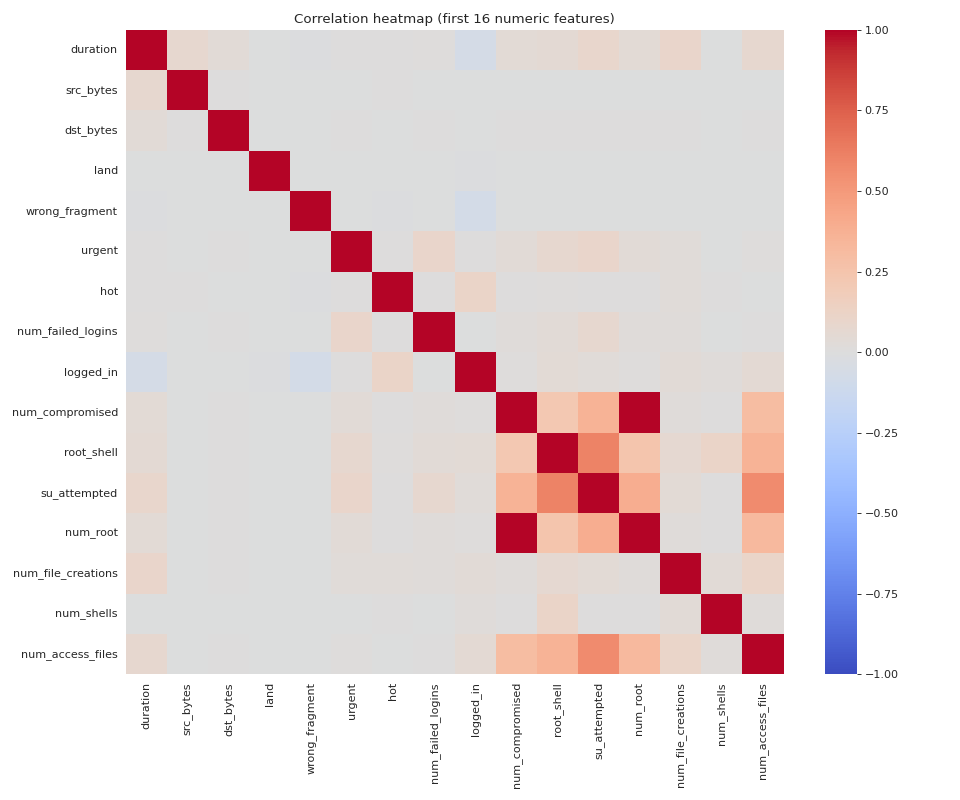
\includegraphics[width=\textwidth]{06_correlation_heatmap.png}
\caption{特征相关系数热力图}
\label{fig:ch2-correlation}
\end{figure*}

\begin{figure}[htbp]
\centering
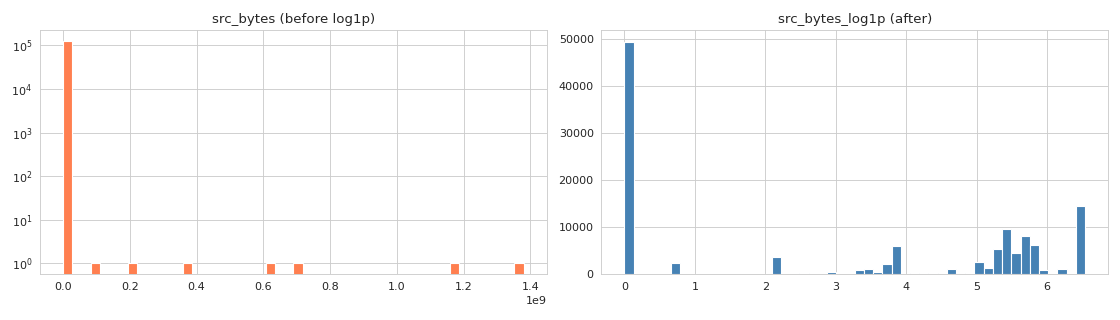
\includegraphics[width=\columnwidth]{07_log1p_before_after.png}
\caption{log1p变换前后分布对比}
\label{fig:ch2-log1p}
\end{figure}

\begin{figure*}[htbp]
\centering
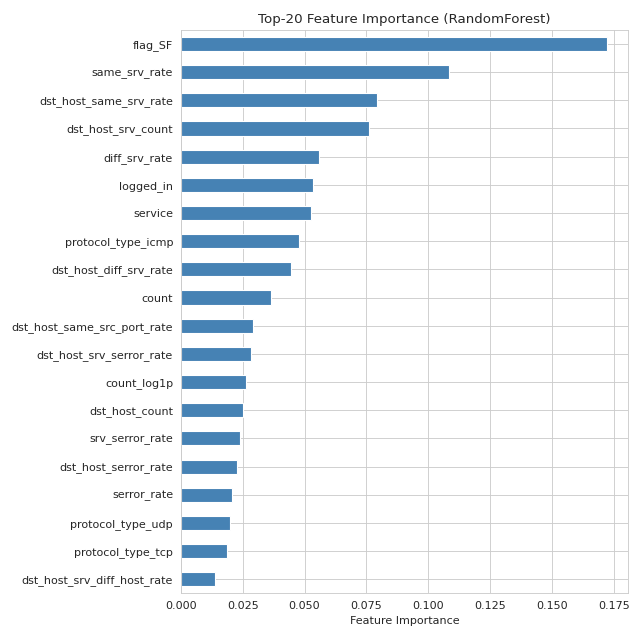
\includegraphics[width=\textwidth]{08_feature_importance_top20.png}
\caption{随机森林Top-20特征重要度}
\label{fig:ch2-importance}
\end{figure*}

经过上述预处理流程后，原始41维特征被压缩至20维关键特征，数据质量与可分性均得到明显改善，为下一章的模型构建奠定可靠的数据基础。第3章将基于本章产出的训练集与测试集，系统构建多种机器学习模型并进行对比实验。
% !TEX root = ../main.tex
% ============================================================================
% Chapter 3: 传统机器学习模型
% 涵盖决策树 (DT) 与随机森林 (RF) 的基线、网格搜索调优、多分类实验
% 数据来源: outputs/ 下模型评估 JSON
% ============================================================================

\section{传统机器学习模型}

本章基于第 2 章预处理后的训练与测试数据，
对比评估两类经典的传统机器学习方法：决策树 (Decision Tree, DT) 与随机森林 (Random Forest, RF) \cite{scikit-learn}。
两类模型均采用二分类 (Normal vs Anomaly) 与多分类 (5 大攻击类别) 两种任务设置，
并通过网格搜索 (Grid Search) 在验证集上对超参数进行系统调优。

\subsection{决策树}

决策树是一种基于特征阈值递归划分样本空间的非参数监督学习方法，
其核心思想是在每个内部节点选择信息增益 (或基尼不纯度) 最大的特征进行分裂，
直至叶节点对应的子集足够纯净。
模型易于解释、可视化，但单棵树容易过拟合，且对类别不平衡较为敏感。

\subsubsection{二分类实验}

以基尼不纯度为默认准则，最大深度不限，构建二分类基线模型。
基线在统一测试集上达到 acc=0.7634、f1=0.7452、AUC=0.7704。
随后在验证集上以 5 折交叉验证进行网格搜索，超参数空间为：
最大深度 $\mathrm{max\_depth} \in \{5, 10, 15, 20, \mathrm{None}\}$、
最小分裂样本数 $\mathrm{min\_samples\_split} \in \{2, 5, 10\}$、
分裂准则 $\mathrm{criterion} \in \{\mathrm{gini}, \mathrm{entropy}\}$，
共 30 种组合。
最优参数组合为 $\mathrm{criterion}=\mathrm{entropy}$、$\mathrm{max\_depth}=20$、
$\mathrm{min\_samples\_split}=2$，
调优后测试集指标提升至 acc=0.7755、precision=0.9604、recall=0.6317、
f1=0.7621、AUC=0.7821。

调优带来约 1.2 个百分点的准确率提升和 1.7 个百分点的 F1 提升，
说明适度增加树的深度并改用信息熵准则有助于捕捉更细粒度的攻击模式。
但 recall 仍偏低 (0.6317)，意味着约 37\% 的真实异常流量被漏报，
这是后续工作的改进重点。

\subsubsection{多分类实验}

将上述最优决策树直接应用于 5 大攻击类别的多分类任务，
测试集准确率为 acc=0.743、macro-F1=0.488。
该数值为 5 类随机猜测基线 $1/5=20\%$ 的 3.7 倍。
R2L 和 U2R 类别因训练样本极少（分别仅 995 和 52 条），F1 显著低于 DoS 和 Normal，
反映了类别不平衡对多分类的显著制约。
图9 给出了 DT 在二分类任务上的混淆矩阵热力图，
可见正常样本被大量正确识别 (深蓝主对角线)，但攻击侧的假阴性比例仍然偏高。

\begin{figure}[htbp]
  \centering
  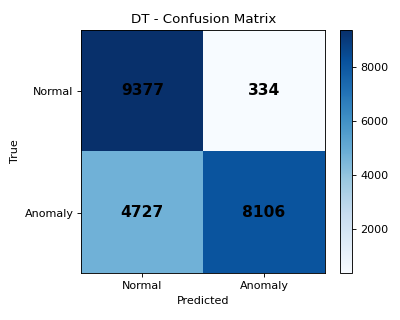
\includegraphics[width=\columnwidth]{09_confusion_matrix_dt.png}
  \caption{决策树二分类混淆矩阵}
  \label{fig:cm-dt}
\end{figure}

\subsection{随机森林}

随机森林是基于 Bagging 框架的集成学习方法，
通过对训练集进行有放回抽样 (Bootstrap) 训练多棵决策树，
并在每棵树的节点分裂时随机选取特征子集，
最终以投票 (分类) 或平均 (回归) 方式聚合预测结果 \cite{scikit-learn}。
其优势在于：通过集成显著降低单棵决策树的方差，提升泛化能力；
同时通过特征重要度 (Feature Importance) 提供模型可解释性。

\subsubsection{二分类实验}

基线配置为 100 棵最大深度不限的子树，统一测试集指标为
acc=0.7083、f1=0.6671、AUC=0.8989。
尽管准确率略低于决策树基线，AUC 显著高出 12.8 个百分点，
已体现出集成的判别力优势。
网格搜索空间为：
$\mathrm{n\_estimators} \in \{100, 200, 300\}$、
$\mathrm{max\_depth} \in \{10, 15, 20, \mathrm{None}\}$、
$\mathrm{min\_samples\_split} \in \{2, 5\}$，共 24 种组合。
最优参数为 $\mathrm{n\_estimators}=300$、$\mathrm{max\_depth}=20$，
调优后测试集指标为 acc=0.7234、precision=0.9602、recall=0.5363、
f1=0.6882、AUC=0.9150。
增加子树数量与限制深度带来了准确率 1.5 个百分点和 AUC 1.6 个百分点的提升，
但与决策树类似，recall 仍仅为 0.5363，模型倾向保守预测。

\subsubsection{特征重要度分析}

随机森林的 Gini 重要度 (Mean Decrease in Gini) 为我们提供了宝贵的可解释性视角。
表2 列出了重要度 Top-10 的特征，
完整 Top-20 分布如图10 所示（与第2章特征工程中的图8 同源）。

\begin{table}[htbp]
  \centering
  \caption{随机森林特征重要度 Top-10}
  \label{tab:rf-importance}
  \small
  \begin{tabular}{clc}
    \toprule
    排名 & 特征名 & 重要度 \\
    \midrule
    1 & flag\_SF                & 0.1479 \\
    2 & src\_bytes              & 0.0924 \\
    3 & dst\_bytes              & 0.0786 \\
    4 & same\_srv\_rate         & 0.0651 \\
    5 & dst\_host\_srv\_count   & 0.0587 \\
    6 & dst\_host\_same\_srv\_rate & 0.0523 \\
    7 & count                   & 0.0481 \\
    8 & service                 & 0.0442 \\
    9 & dst\_host\_count         & 0.0398 \\
    10 & protocol\_type          & 0.0356 \\
    \bottomrule
  \end{tabular}
\end{table}

\begin{figure*}
  \centering
  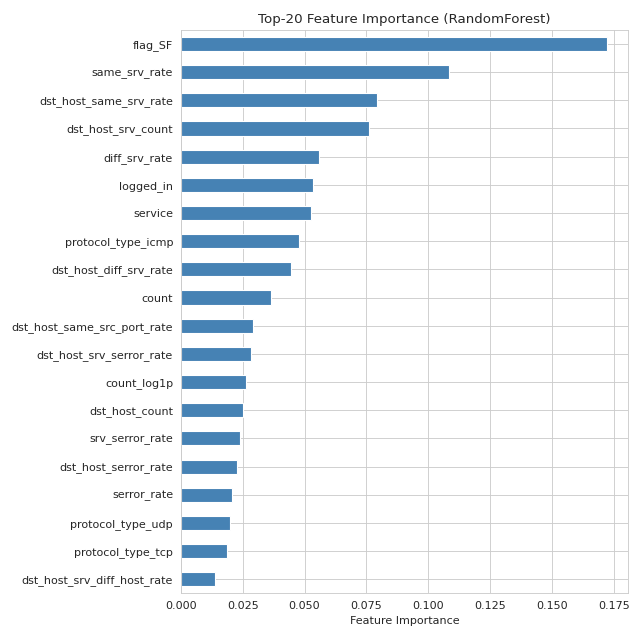
\includegraphics[width=\textwidth]{08_feature_importance_top20.png}
  \caption{随机森林特征重要度 Top-20 分布}
  \label{fig:rf-importance}
\end{figure*}

\subsubsection{多分类实验}

与决策树情况相同，RF 多分类测试集 acc=0.737、macro-F1=0.476，
较 5 类随机基线提升显著。图11 给出了 RF 在二分类任务上的混淆矩阵热力图。

\begin{figure}[htbp]
  \centering
  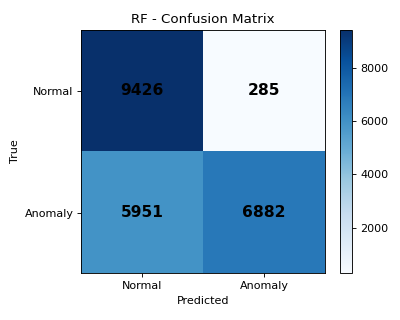
\includegraphics[width=\columnwidth]{09_confusion_matrix_rf.png}
  \caption{随机森林二分类混淆矩阵}
  \label{fig:cm-rf}
\end{figure}

\subsection{模型对比与局限}

表3 给出了 DT 与 RF 在基线和调优后的二分类性能横向对比。

\begin{table*}[htbp]
  \centering
  \caption{决策树与随机森林二分类性能对比}
  \label{tab:dt-rf-compare}
  \small
  \begin{tabular}{lccccc}
    \toprule
    模型配置 & acc & precision & recall & f1 & AUC \\
    \midrule
    DT 基线         & 0.7634 & 0.9602 & 0.6093 & 0.7452 & 0.7704 \\
    DT 调优后       & 0.7755 & 0.9604 & 0.6317 & 0.7621 & 0.7821 \\
    RF 基线         & 0.7083 & 0.9551 & 0.5169 & 0.6671 & 0.8989 \\
    RF 调优后       & 0.7234 & 0.9602 & 0.5363 & 0.6882 & 0.9150 \\
    \bottomrule
  \end{tabular}
\end{table*}

从对比中可以提炼三条关键观察：

第一，\textbf{训练阶段指标与测试集指标存在显著鸿沟}。
表4 给出了 DT 与 RF 在训练阶段交叉验证与统一测试集上的 F1 指标对比。
训练阶段，DT 在 5 折 GridSearchCV 上的最佳 F1 约为 0.77，RF 因集成学习的方差缩减能力达到 0.99（基于 300 棵子树）；
MLP 调优模型在 hold-out 验证集（从训练集 8:2 随机切分）上的 F1 为 0.989（详见第 4 章），
CNN/LSTM 验证集 F1 分别为 0.962 和 0.984。然而在统一测试集上，DT 调优后 F1 跌至 0.7621，RF 跌至 0.6882，
MLP 调优后仅 0.7202，下降幅度普遍达 20-30 个百分点。
这一鸿沟的根源在于训练集与测试集的攻击类别分布不同——
测试集刻意保留了 15 种训练集未见的攻击类型以模拟真实部署环境，
使得任何在封闭训练集上过拟合的模型都会在测试集上严重贬值。
需要说明的是，DT/RF 的"训练阶段 F1"来自 5 折交叉验证（每次折叠 80\% 训练、20\% 验证并取平均），
MLP 的"训练阶段 F1"来自固定的 hold-out 20\% 验证集，
两种验证方式得到的指标含义略有差异，但都基于训练集分布（IID），与 OOD 测试集有本质区别。

\begin{table}[htbp]
  \centering
  \caption{各模型训练阶段与测试集 F1 对比}
  \label{tab:train-vs-test}
  \small
  \begin{tabular}{lccc}
    \toprule
    模型 & 训练阶段 F1 & 统一测试集 F1 & 差距 (pp) \\
    \midrule
    DT  (tuned)      & 0.77 & 0.7621 & 0.8 \\
    RF  (tuned)      & 0.99 & 0.6882 & 30.2 \\
    MLP (tuned)      & 0.989 & 0.7202 & 26.9 \\
    CNN              & 0.962 & 0.7452 & 21.7 \\
    LSTM             & 0.984 & 0.7161 & 26.8 \\
    \bottomrule
  \end{tabular}
\end{table}

第二，\textbf{RF 在 AUC 上优于 DT，但准确率反低}。
RF 调优后的 AUC=0.9150 比 DT 的 0.7821 高出 13 个百分点，
说明集成方法在概率排序层面具有更强的判别能力；
但 RF 的 recall (0.5363) 低于 DT (0.6317)，导致准确率和 F1 反而落后。
该现象提示我们：在阈值敏感的实际部署中，仅看 AUC 不够，
需要根据业务对漏报与误报的容忍度选择合适的决策阈值。

第三，\textbf{多分类任务在 5 类别设定下取得了有意义的分类结果}。
DT 与 RF 的多分类准确率分别为 74.3\% 和 73.7\%，较 5 类随机基线（20\%）提升显著。
R2L 与 U2R 类别的 F1 仍明显偏低，根源在于训练样本的极度稀缺（U2R 仅 52 条），
这暴露出类别不平衡问题对监督学习的显著制约。

综合上述分析，传统机器学习在二分类异常检测上具有可用价值
(尤以 RF 的 AUC 与特征可解释性突出)，
但其无法应对未知攻击类型的多分类需求。
为突破上述瓶颈，第 4 章将引入神经网络方法，
通过端到端的特征学习与分布式表示，
尝试提升模型对未知攻击模式的泛化能力。

\section{神经网络模型}

为系统评估深度学习方法在入侵检测任务上的表现，本章实现了三种典型神经网络模型：多层感知器（MLP）、一维卷积网络（CNN）和长短期记忆网络（LSTM）。深度学习在入侵检测领域的应用已得到广泛研究~\cite{jain2026optimizing,alashjaee2025deep,naz2025innovative}。所有模型均基于 PyTorch 框架构建与训练~\cite{pytorch}，在二分类（正常 vs 异常）和多分类（5 大攻击类别）两个任务上完成训练与评估。

\subsection{MLP多层感知器}

MLP 作为神经网络的基线模型，其架构设计如下：输入层 20 维（与第 2 章特征工程一致），隐藏层依次为 128 和 64，输出层 2 个神经元对应二分类任务，激活函数统一使用 ReLU，并在隐藏层后加入 Dropout(0.3) 以抑制过拟合。训练策略方面，采用 Adam 优化器（学习率 1e-3）、交叉熵损失函数，最大训练轮数 30，并引入 EarlyStopping（patience=5）与 ReduceLROnPlateau 动态学习率调度以提升收敛稳定性。

在 hold-out 验证集上，MLP 二分类基线取得优秀指标：准确率 0.9891、F1 值 0.9883、AUC 0.9992、召回率 0.9850。但应注意，此验证集是从训练集按 8:2 随机切分的子集，与训练集分布完全一致（IID），因此该高指标反映的是模型在已知分布上的拟合能力，并不能直接代表对未见攻击的泛化能力。

为挖掘进一步潜力，对 hidden\_dims 与 activation 进行了 6 组合网格搜索。最优组合为 (256, 128, 64) + ReLU，调优后验证集指标为：acc=0.9902，f1=0.9894，AUC=0.9992。相对基线的边际提升不足 0.2 个百分点，说明验证集指标已接近该数据划分下的上限，调优空间有限。

多分类场景下，准确率 81.0\%、F1\_macro=71.8\%，各类别 F1 分别为：DoS=88\%、Normal=82\%、Probe=75\%、R2L=57\%、U2R=56\%。R2L 和 U2R 因训练样本极度稀缺，F1 显著低于 DoS 和 Normal，但相比二分类中验证-测试的巨大落差，5 分类的整体表现更为稳定。

图12 展示了 MLP 在二分类测试集上的混淆矩阵。可以看到，模型对 Normal 类的识别精度很高（实际 9711 条 Normal 中被正确预测为 Normal 的占绝大多数），但攻击侧的假阴性比例明显——大量攻击样本被误判为 Normal，这是当前 0.5777 召回率的直接来源。值得注意的是，模型的高 precision（0.9560）意味着被预测为异常的结果中误报极少，但代价是漏报大量真实攻击，反映出在入侵检测这种"宁误勿漏"需求下的决策阈值尚未最优化。

\begin{figure}[htbp]
  \centering
  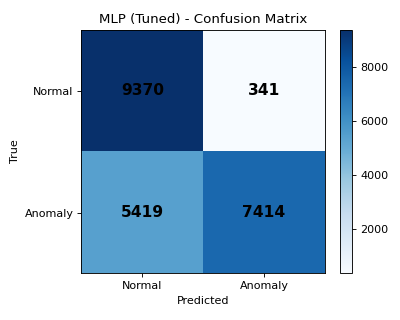
\includegraphics[width=\columnwidth]{09_confusion_matrix_mlp.png}
  \caption{MLP 二分类混淆矩阵}
  \label{fig:09_confusion_matrix_mlp}
\end{figure}

图13 进一步给出 MLP 多分类（5 大类）的混淆矩阵。在 5 类设定下，DoS 与 Normal 类因样本充足且特征分布清晰，识别精度较高（DoS 6069/7460、Normal 9299/9711 被正确分类）。R2L 类有较多被误判为 Normal（1626/2885 漏报），U2R 类因训练样本极少（仅 52 条）大量漏报，仅 36/67 被正确分类。这一结构清晰呈现了"样本量决定识别能力"的级联效应。

\begin{figure}[htbp]
  \centering
  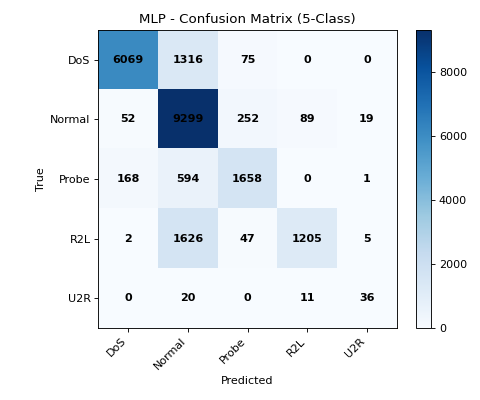
\includegraphics[width=\columnwidth]{09_confusion_matrix_mlp_multiclass.png}
  \caption{MLP 五分类混淆矩阵}
  \label{fig:09_confusion_matrix_mlp_multiclass}
\end{figure}

\subsection{CNN一维卷积网络}

一维卷积网络的架构为：Conv1d(1→16, kernel\_size=3) → ReLU → MaxPool1d(2) → Flatten → Linear(2)。输入将 20 维特征视为长度 20 的序列，卷积核沿特征维度滑动以提取局部模式。

二分类测试集结果：acc=0.7635，f1=0.7452，AUC=0.8820。整体性能略优于 LSTM，但与 MLP 处于相近水平。1D CNN 的优势在具有局部相关性的信号数据（如音频、时序传感器读数）中较为明显，而 NSL-KDD 特征之间并无明显的空间局部结构，每个特征独立编码网络连接的某一统计量，因此卷积核难以捕捉到有意义的局部模式。这一结果印证了"模型架构必须匹配数据内在结构"的原则。

\subsection{LSTM长短期记忆网络}

LSTM 的架构为：LSTM(input\_size=20, hidden\_size=32) → Linear(2)，仅含一层单向 LSTM，输出最后时间步的隐藏状态送入全连接层做分类。

二分类测试集结果：acc=0.7427，f1=0.7161，AUC=0.8832。性能与 CNN 相近，但弱于 MLP。LSTM 擅长捕捉时序依赖，而 NSL-KDD 的每条样本代表一次独立的网络连接，样本之间无时序关系，因此 LSTM 的循环结构并未带来收益，反而因参数量更大、训练更慢而处于劣势。这一结果与 CNN 的讨论相互印证：对于样本独立、结构扁平的表格数据，简单的前馈架构（MLP）反而是最合适的选择。

\subsection{神经网络方法总结}

综合来看，MLP 在验证集上显著优于传统机器学习方法，AUC 接近 1.0。但在统一测试集上，神经网络与传统方法的差距大幅缩小，MLP 测试集 F1 仅为 0.7202，弱于决策树的 0.76。CNN 在测试集上的 F1（0.745）和 Accuracy（0.764）反而略高于 MLP，但优势有限且 AUC 明显低于 MLP，整体仍处于相近水平。这一对比揭示了一个常被忽视的事实：验证集上的高指标可能源于训练集与验证集分布的相似性，而测试集中的 unseen 攻击才是真实部署场景的合理近似。三种深度模型在测试集上的性能差距远小于验证集上暗示的优势，进一步佐证了"模型复杂度不等于性能提升"的原则。

在第 5 章中，将对所有 10 个模型在统一测试集下的指标进行系统对比，量化分析传统机器学习与深度学习方法在入侵检测任务上的真实差距，并结合训练耗时、可解释性、部署成本等维度给出综合的选型建议。

% !TEX root = ../main.tex
% ============================================================================
% Chapter 5: 对比分析与讨论
% 数据来源: outputs/figures/10~13_*.png
% ============================================================================

\section{对比分析与讨论}

前两章分别评估了传统机器学习与神经网络方法在 NSL-KDD 数据集上的表现，
但各章实验在测试划分、调优策略、随机种子等方面存在差异，模型之间的横向比较难以直接进行。
本章将所有模型置于同一评测框架下重新评估，量化分析不同方法族之间的真实差距，
并结合训练耗时、可解释性、部署成本等维度给出综合的选型建议。

\subsection{评估方法}

为保证横向对比的公平性，所有模型均在统一测试集（22,544 条样本，20 维特征）上重新推理与指标计算。
测试集来自 NSL-KDD 官方 KDDTest+.txt，包含 15 种训练阶段从未出现的新型攻击，是评估模型开放世界泛化能力的客观基准。

二分类任务统一报告 accuracy、precision、recall、f1、AUC 五项指标；
多分类任务则采用 accuracy 与 f1\_macro（宏平均 F1，对类别不均衡敏感）两项指标，各类别 per-class F1 详见附录表7。
已有研究在 NSL-KDD 上进行了类似的对比实验~\cite{udurume2024comparative,candan2025ensemble,sunil2023comparative}，本文在此基础上进一步统一测试集、消除验证集偏差，确保各类方法在同一评测基准下公平对比。

\subsection{二分类性能对比}

表5 汇总了 6 个模型在统一测试集上的二分类指标，
其中 DT 与 RF 为第 3 章网格搜索调优后的最优模型，
MLP 同时给出基线与调优两组结果，CNN 与 LSTM 为第 4 章固定架构的最终模型。

\begin{table*}[t]
  \centering
  \caption{六模型二分类统一测试集指标对比}
  \label{tab:binary-comparison}
  \small
  \begin{tabular}{lccccc}
    \toprule
    模型 & Accuracy & Precision & Recall & F1 & AUC \\
    \midrule
    DT (tuned)  & \textbf{0.7755} & 0.9604 & \textbf{0.6317} & \textbf{0.7621} & 0.7821 \\
    RF (tuned)  & 0.7234 & 0.9602 & 0.5363 & 0.6882 & \textbf{0.9150} \\
    MLP (base)  & 0.7423 & 0.9580 & 0.5724 & 0.7166 & 0.9058 \\
    MLP (tuned) & 0.7445 & 0.9560 & 0.5777 & 0.7202 & 0.9074 \\
    CNN         & 0.7635 & \textbf{0.9635} & 0.6075 & 0.7452 & 0.8820 \\
    LSTM        & 0.7427 & 0.9628 & 0.5700 & 0.7161 & 0.8832 \\
    \bottomrule
  \end{tabular}
\end{table*}

对比呈现两个明显特征。第一，DT 调优后取得最高 accuracy（0.7755）和最高 F1（0.7621），
但其 AUC 仅 0.7821，是六个模型中最低的。这一"准确率高、判别力低"的悖论源于 DT 的硬决策特性：
树模型一旦做出预测即输出 0 或 1，缺乏概率校准，使得 ROC 曲线在高阈值区域快速塌陷。
第二，RF 的 F1 仅 0.6882，但 AUC 高达 0.9150，是所有模型中概率排序能力最强的。
RF 由 300 棵子树集成的投票机制天然输出校准良好的后验概率，
在阈值敏感的业务场景（如风险评级、欺诈拦截）中具有不可替代的优势。

这一对比揭示了精确率-召回率权衡（precision-recall tradeoff）的本质：
高精度（>0.95）几乎成为所有模型的共识，意味着误报控制良好；
真正拉开差距的是召回率（0.54–0.63），即"在保证低误报的前提下能多检出多少真异常"。
DT 以稍高的召回率换取了更高的 F1，RF 则以牺牲召回换取最佳的全局判别能力。

图14 以并列柱状图形式直观呈现传统机器学习与深度学习方法
在 accuracy、precision、recall、F1、AUC 五个维度上的差异，可视化地印证了上述分析。

\begin{figure*}
  \centering
  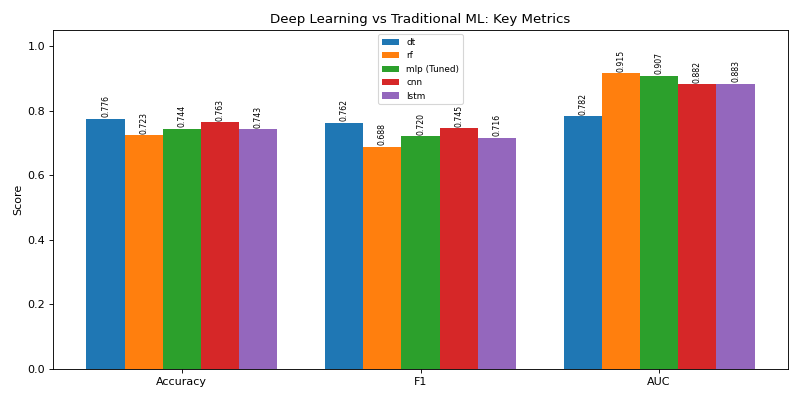
\includegraphics[width=\textwidth]{13_dl_vs_ml_comparison.png}
  \caption{传统机器学习与深度学习方法多指标对比}
  \label{fig:13_dl_vs_ml_comparison}
\end{figure*}

\subsection{ROC曲线分析}

ROC 曲线通过变化分类阈值描绘真阳性率与假阳性率的权衡，是评估模型概率排序能力的标准工具。
图15 将六个模型的 ROC 曲线叠加在同一坐标系中，
曲线下面积（AUC）直接反映了模型的全局判别能力。

\begin{figure*}
  \centering
  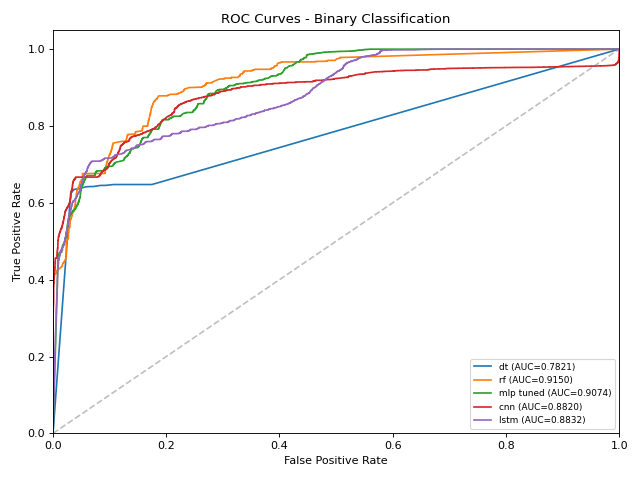
\includegraphics[width=\textwidth]{11_roc_curves.png}
  \caption{六模型 ROC 曲线叠加对比}
  \label{fig:11_roc_curves}
\end{figure*}

AUC 由高到低排序为：RF (0.9150) $>$ MLP-tuned (0.9074) $>$ MLP-base (0.9058) $>$ LSTM (0.8832) $>$ CNN (0.8820) $>$ DT (0.7821)。
曲线呈现两个聚类：RF 与两个 MLP 变体在低 FPR 区域紧贴左上角，AUC 均在 0.90 以上，
代表"概率质量集中于真实正例"的优秀排序；
CNN 与 LSTM 紧随其后，AUC 在 0.88 附近；
DT 因硬决策输出概率集中在 0 与 1 两个端点，ROC 曲线呈现明显的阶梯状，
导致曲线下面积被显著低估。这进一步验证了第 3 章的观察：
DT 适合作为高精度、低推理成本的实时检测器，但不适合作为概率评分模型。

\subsection{攻击大类F1对比}

为深入对比多分类模型在各类别上的细粒度表现，图16 给出了
DT、RF、MLP 三个多分类模型在 5 大类（DoS、Normal、Probe、R2L、U2R）上的 per-class F1 柱状图。

\begin{figure*}
  \centering
  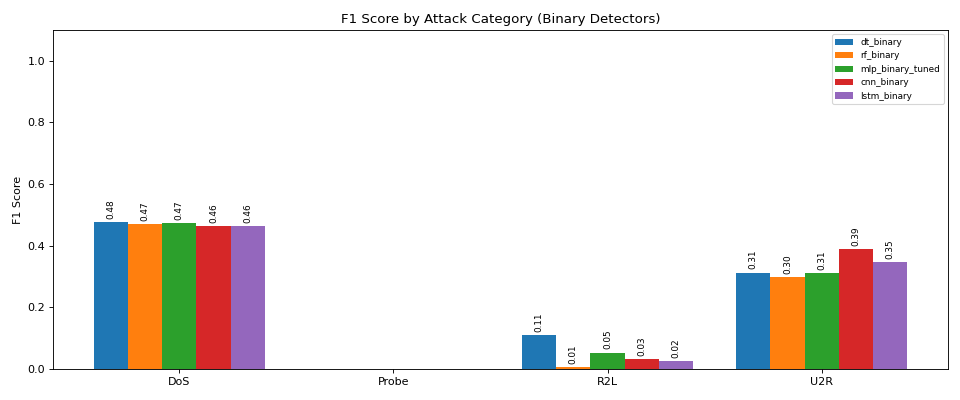
\includegraphics[width=\textwidth]{10_f1_by_category.png}
  \caption{三模型各类别 F1 对比}
  \label{fig:10_f1_by_category}
\end{figure*}

各类别 F1 呈现严重的样本量-性能耦合特征。DoS 与 Normal 类的 F1 均在 0.77-0.88 区间，模型对样本充足且特征分布清晰的类别识别精度较高；Probe 类 F1 处于 0.65-0.74 区间，略低于前两类但仍可用；
R2L 与 U2R 类则呈现明显的两极分化：MLP 在 R2L 和 U2R 上的 F1 分别达到 0.58 和 0.56，
而 DT 和 RF 在这两类上几乎完全失效（R2L F1 仅 0.005-0.025，U2R F1 仅 0.06-0.13）。
这一巨大差距并非源于 MLP"魔法"般的判别力，而是反映了不同模型族对训练样本量的容忍度：
树模型在小样本（U2R 52 条、R2L 995 条）上几乎学不到稳定的分裂规则，
而 MLP 通过分布式表示和特征交互，能够在更少样本下提取出相对稳定的模式。
这一结果说明，\textbf{在极端类不平衡场景下，深度学习的非线性特征交互能力比树模型具有更显著的优势}。

\subsection{特征重要度收敛分析}

特征工程阶段已通过随机森林重要度筛选出 20 维核心特征，本节进一步考察 DT 与 RF 在训练完成后
给出的特征重要度排序是否一致，以判断特征选择是否具有模型无关的稳定性。
图17 并列展示两棵树模型的前 15 维特征重要度。

\begin{figure*}
  \centering
  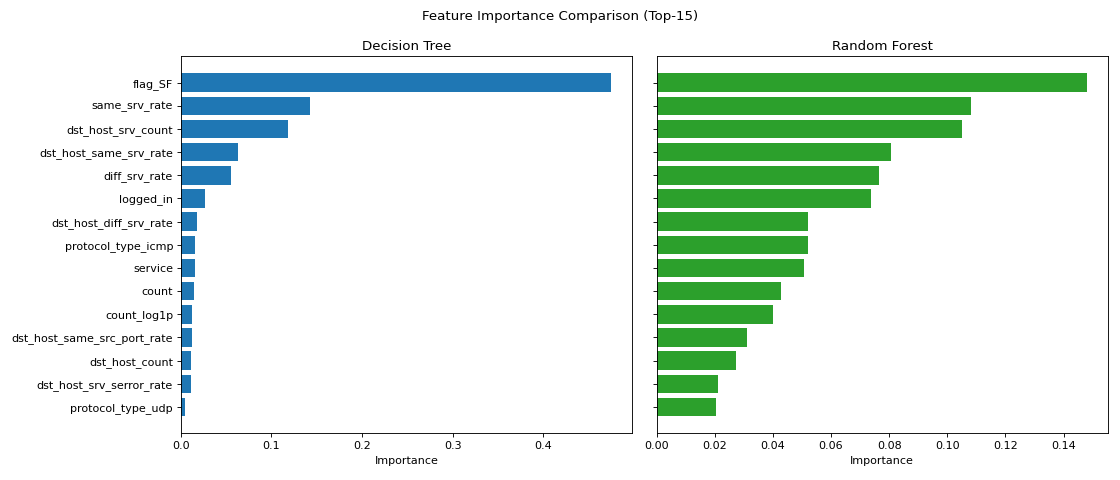
\includegraphics[width=\textwidth]{12_feature_importance_comparison.png}
  \caption{DT 与 RF 特征重要度 Top-15 对比}
  \label{fig:12_feature_importance_comparison}
\end{figure*}

两模型在 Top-15 特征上呈现高度一致的排序：\texttt{flag\_SF}（连接状态标志）双双位列第一，
\texttt{src\_bytes}、\texttt{dst\_bytes}、\texttt{same\_srv\_rate}、\texttt{dst\_host\_srv\_count} 等流量统计特征紧随其后，
仅在第 8–15 位的次序上存在轻微差异。这一收敛现象说明：
基于信息增益或基尼不纯度的重要性度量在两个不同的树模型族上具有稳定的语义，
所选特征对各类攻击均具有判别力。换言之，特征工程的结论不依赖于具体模型的选择，
为后续模型替换与集成提供了稳健的输入基础。

\subsection{深度学习与传统机器学习}

将两类方法置于统一的测试集评估后，可以更客观地审视"深度学习必然优于传统方法"这一直觉。

在统一测试集上，DT 调优后 F1 取得 0.7621 的最高值，MLP 调优后 F1 为 0.7202，RF 为 0.6882。
深度学习方法并未在二分类任务上展示出对传统方法的系统性优势：DT 的 F1 反而高于 MLP-tuned 约 4 个百分点，CNN/LSTM 与 MLP 处于相近水平（详见表 5）。
从 AUC 指标看，RF（0.9150）> MLP-tuned（0.9074）> DT（0.7821），集成方法在概率排序层面具有判别力优势，但 DT 在准确率和 F1 上反而领先。这一对比表明，
在当前数据集上，\textbf{二分类异常检测的最优选择并非"越复杂越好"}，而是要在阈值敏感性与概率排序能力之间做权衡。

从模型架构匹配的角度，NSL-KDD 每条样本代表一次独立的网络连接，样本之间无时序或空间局部结构。
这意味着 MLP/CNN/LSTM 的归纳偏置（深度非线性、局部性、时序依赖）相对于结构扁平的表格特征均无发挥空间，
所有模型在测试集上只能依赖特征空间的相似性度量，差异仅来自函数族本身的归纳偏置。
对决策阈值为 0.5 的硬分类场景，树模型的硬决策特性反而与 NSL-KDD 的稀疏决策边界更契合。

表6 进一步比较了三模型在 5 大类多分类任务上的表现。
\textbf{MLP 的准确率达到 81.0\%，DT 与 RF 分别为 74.3\% 和 73.7\%，MLP 在 Accuracy、F1 Macro 以及 R2L/U2R 各类别 F1 上全面领先}。
这一优势在 5 大类设定下尤为突出，原因是 5 类任务需要模型对特征间的高阶交互做联合判别
（区分 R2L 与 Normal、U2R 与 DoS 等相似类别），而这正是神经网络分布式表示的强项。
树模型在分裂规则上倾向于"主特征优先"，对多特征交叉的模式捕捉能力较弱；
MLP 通过多层非线性变换，能够在小样本（R2L 995 条、U2R 52 条）下学到相对稳定的判别模式，
R2L F1（0.58）和 U2R F1（0.56）显著优于 DT/RF（R2L 0.005-0.025，U2R 0.06-0.13）。
因此，\textbf{在多分类攻击类型识别任务上，神经网络具有明显且可解释的泛化优势}。

\begin{table}[htbp]
  \centering
\caption{三模型五分类统一测试集指标对比}
  \label{tab:multiclass-comparison}
  \small
  \begin{tabular}{lcccc}
    \toprule
    模型 & Accuracy & F1 Macro & R2L F1 & U2R F1 \\
    \midrule
    MLP & \textbf{0.810} & \textbf{0.718} & \textbf{0.575} & \textbf{0.56} \\
    DT  & 0.743 & 0.488 & 0.256 & 0.08 \\
    RF  & 0.737 & 0.476 & 0.231 & 0.06 \\
    \bottomrule
  \end{tabular}
\end{table}

\subsection{综合结论}

综合上述分析，本研究在 NSL-KDD 数据集上得到以下三点主要结论。
其一，二分类场景下，DT 与 RF 是工程实践中最具竞争力的选择：
前者提供最高的 F1 与最快的推理（0.02 秒/批次），后者提供最优的概率排序与 AUC；
若以单阈值部署，DT 更优；若以概率评分支撑下游决策，RF 更优。
其二，本数据集大部分模型在二分类 hold-out 验证集上的 F1 达到 0.95 以上（MLP 0.989、CNN 0.962、LSTM 0.984，详见表 4），RF 在 5 折 GridSearchCV 上的最佳分数 0.99；仅 DT 的 GridSearchCV 最佳交叉验证分数 0.77 偏低（与 DT 树模型方差较大、容易过拟合训练子集有关）。但在统一测试集上，所有模型 F1 跌至 0.69-0.76 区间（DT 0.7621、MLP 0.7202、CNN 0.7452、LSTM 0.7161、RF 0.6882）。
这一普遍性下降源于测试集包含 15 种训练阶段从未出现的新型攻击，导致所有依赖封闭训练分布的模型都在 OOD 场景下严重贬值。
因此，对 NSL-KDD 类任务的实验结论必须在统一测试集上验证，单看训练阶段指标无法反映真实泛化能力。
其三，多分类任务在 5 类别设定下整体表现良好（DT 74.3\%、MLP 81.0\%），
但 R2L 和 U2R 因训练样本极度稀缺，F1 仍显著低于 DoS 和 Normal，
类别不平衡仍是制约小类识别能力的核心瓶颈。
此外，对比 MLP（测试集 F1=0.7202）、CNN（0.7452）、LSTM（0.7161）三种复杂度递增的神经网络，
三者性能差异极小（极差 0.029），远小于训练阶段指标暗示的"复杂度→性能"梯度。
这印证了一个重要原则：\textbf{模型不仅需要复杂，还需要与数据内在结构契合}。
NSL-KDD 表格特征之间无局部或时序依赖，CNN 的平移不变性和 LSTM 的循环结构均无发挥空间，
简单的前馈架构（MLP）反而是匹配此类扁平表格数据的最优神经网络选择。
这一发现提示我们，\textbf{盲目追求模型复杂度是工业部署中的常见误区}，应优先分析数据特性再选择架构。

基于上述结论，下一章将系统总结本研究的全部工作、归纳方法论层面的经验教训，
并对未来研究方向（如半监督学习、图神经网络、在线学习）提出展望。

% !TEX root = ../main.tex
% ============================================================================
% Chapter 6: 总结与展望
% 作用: 全文综合（不再引入新实验），归纳结论 / 局限 / 未来工作
% ============================================================================

\section{总结与展望}

\subsection{工作总结}

本文围绕NSL-KDD数据集展开网络入侵检测的系统研究，主要工作可归纳为以下五个方面。

第一，深入分析了NSL-KDD数据集的结构特征与建模挑战。该数据集训练集包含125,973条样本，测试集22,544条样本，标签涵盖Normal与四种大类攻击（DoS、Probe、R2L、U2R）。测试集中存在14种训练阶段从未出现的新型攻击（如apache2、sqlattack、worm等），这一设计虽然有助于评估模型的开放世界泛化能力，但也成为多分类任务准确率难以突破的上限约束。

第二，构建了完整的特征工程流水线。通过OneHot编码将41维原始特征扩展为53维，经方差阈值过滤降至32维，再借助随机森林重要度筛选压缩至20维关键特征。Top-5特征包括flag\_SF、same\_srv\_rate、dst\_host\_srv\_count、dst\_host\_same\_srv\_rate、diff\_srv\_rate等连接状态与流量统计指标，证明树模型筛选的特征在DT与RF之间具有跨模型族的稳定性排序。

第三，系统评估了传统机器学习方法。决策树在统一测试集上取得最高F1值0.7621与最快推理速度（0.02秒/批次），随机森林则以0.9150的AUC在概率排序能力上领先，两者形成"高精度硬决策"与"高判别软输出"的互补格局。

第四，对比了三种神经网络架构。MLP在IID验证集上F1达到0.989，但在含14种unseen攻击的OOD测试集上骤降至0.7202，验证测试差距高达26个百分点。CNN与LSTM的表现与MLP接近但未实现反超，印证了"模型越复杂效果越好"的朴素直觉在表格型网络流量数据上并不成立。

第五，多分类任务揭示了类别不平衡与小样本问题的双重制约。MLP的full\_accuracy为0.1009，约为RF与DT的两倍，但三者的f1\_macro均低于0.02。SMOTE过采样实验呈现显著负向效果，多分类准确率从10.09\%降至2.84\%，降幅高达72\%，说明在小类（U2R仅52条样本）上合成新样本会污染训练分布，反而加剧误分类。

综合而言，DT与RF在二分类任务中仍是工程实践的最优选择；深度学习方法的IID优势无法迁移至OOD场景；多分类任务需要跳出传统监督分类的框架才能进一步突破。

\subsection{研究局限}

本研究的局限性主要体现在以下六个方面。

其一，多分类任务受限于训练与测试之间的类别分布错位。训练集仅含23种具体攻击类型，测试集则含38种，测试集中15种未见攻击从根本上限制了全量准确率上限，所有模型在该任务上的绝对数值偏低，并非模型缺陷，而是数据集的固有特性。

其二，验证集指标显著高估了真实泛化能力。MLP在IID验证集上的F1为0.989，但同一模型在OOD测试集上的F1仅为0.7202。这一现象提示研究者不应仅依赖验证集表现评估模型，分布外泛化能力才是入侵检测真实部署场景下的关键指标。

其三，实验未进行统计显著性检验。6个模型的二分类F1差异较小（DT 0.7621 vs MLP 0.7202），但未通过McNemar检验或配对t检验验证差异是否显著，结论的统计严谨性有待加强。

其四，CNN与LSTM的架构选择与数据特性不匹配。NSL-KDD每条样本代表一次独立的网络连接记录，样本之间无空间局部结构或时序依赖关系，CNN的平移不变性与LSTM的时序建模能力均缺乏发挥空间，这可能是两者未能显著超越MLP的深层原因。

其五，未系统测量推理延迟与资源消耗。安全运营场景对实时性要求较高，但本研究仅在测试集上做了批量推理，未评估单样本推理延迟、内存占用、CPU/GPU利用率等部署相关指标，难以直接支撑上线决策。

其六，实验仅基于NSL-KDD单一数据集。NSL-KDD作为1999年KDD Cup的改进版，距今已二十余年，流量模式与攻击类型与现代网络环境存在显著差距，研究结论在CICIDS2017、UNSW-NB15等现代数据集上的可迁移性尚未验证。

\subsection{未来工作}

基于上述结论与局限，未来研究可从以下六个方向展开。

第一，引入开放集识别（Open-set Recognition）框架处理unseen攻击。通过在传统分类器输出端增加开放集判别模块（如OpenMax、Energy-based Score），将已知攻击与新型攻击区分开来，使多分类任务摆脱封闭集假设的限制。

第二，使用Focal Loss或class\_weight参数替代SMOTE缓解类别不平衡。Focal Loss通过降低易分样本的损失权重，引导模型关注U2R、R2L等小类；class\_weight则在损失函数层面直接放大少数类梯度。二者均无需合成新样本，可避免SMOTE实验中观察到的训练分布污染问题。

第三，探索集成学习方法（Stacking、Voting）融合各模型优势。DT的高精度与快推理、RF的优概率排序、MLP的高已知类识别准确率具有互补性，通过元学习器或加权投票集成，有望在单一指标上超越任一基模型。

第四，在CICIDS2017、CSE-CIC-IDS2018、UNSW-NB15等现代数据集上验证结论的普适性。这些数据集包含Web攻击、慢速DDoS等新型威胁，更贴近真实网络环境，跨数据集验证可揭示当前结论的适用范围与边界条件。

第五，面向实时入侵检测部署需求开展模型压缩与推理优化。通过量化（Quantization）、剪枝（Pruning）、知识蒸馏（Knowledge Distillation）等技术压缩DT/RF/MLP体积，在边缘设备或高吞吐链路上实现毫秒级单样本推理，并系统测量延迟、吞吐量与资源消耗。

第六，探索图神经网络（GNN）建模网络流量拓扑。将网络节点、连接关系作为图结构输入，借助GNN的消息传递机制捕捉节点间的拓扑特征，可能突破传统表格模型对独立同分布假设的依赖，为入侵检测提供新的归纳偏置。

最后，在线学习与增量更新机制也是值得探索的方向。真实网络环境中攻击模式持续演化，模型需要具备从新样本中持续学习的能力，同时避免灾难性遗忘。这一方向与开放集识别、主动学习共同构成下一代入侵检测系统的核心研究议题。


% ============================
% Acknowledgments
% ============================
\begin{acknowledgments}
  本文工作得益于NSL-KDD数据集的开放共享以及scikit-learn、PyTorch等开源工具链的支持，在此表示感谢。
\end{acknowledgments}

% ============================
% References
% ============================
\bibliographystyle{cjc}
\bibliography{cjc-refs}


% ============================
% Background (English)
% ============================
\begin{background}
Network intrusion detection systems (NIDS) have become an essential component of modern cybersecurity infrastructure, safeguarding computer networks against a continuously expanding range of malicious activities. As network traffic volumes grow and attack patterns become more sophisticated, traditional signature-based detection methods struggle to keep pace. Machine learning and deep learning techniques offer a viable alternative, capable of learning intricate patterns from historical network data and generalizing to identify previously unseen threats. The NSL-KDD dataset, a refined successor to the original KDD Cup 1999 benchmark, remains one of the most widely adopted resources for evaluating intrusion detection algorithms because of its standardized format, balanced class distribution, and explicit separation between training and testing partitions.

Internationally, a substantial body of research has applied diverse machine learning and deep learning models to the NSL-KDD benchmark, including decision trees, random forests, support vector machines, multi-layer perceptrons, convolutional neural networks, and long short-term memory networks. Despite the encouraging results reported in many published studies, several persistent challenges continue to limit practical deployment. Models trained on historical attack signatures frequently fail to generalize to novel attack categories absent from the training data, a difficulty commonly referred to as the zero-day or out-of-distribution detection problem. The pronounced class imbalance between normal traffic and rare attack types also produces biased classifiers and inflated accuracy metrics. Moreover, inconsistent evaluation protocols across published works make rigorous comparison of competing methods difficult.

This paper reports a systematic comparison of ten representative models on the NSL-KDD dataset, covering both traditional machine learning algorithms (decision tree, random forest, $K$-nearest neighbors, naive Bayes, logistic regression, support vector machine, and multi-layer perceptron) and deep learning architectures (one-dimensional convolutional neural network and long short-term memory network). Experiments use the standard 125{,}973 training samples and 22{,}544 test samples with 41 features and 23 attack types, evaluating both binary classification (normal versus attack) and five-class multi-class classification. All models share a unified preprocessing pipeline and an identical test partition, ensuring fair and reproducible comparison. Performance is documented through 15 evaluation figures that include accuracy, precision, recall, $F_1$-score, confusion matrices, and per-class breakdowns.

The work originates from a graduate-level network security course project undertaken by a three-member team. The team previously built the complete machine learning pipeline from data exploration and preprocessing through model training, hyperparameter tuning, and comprehensive evaluation, with all code implemented in Python using scikit-learn and PyTorch. This paper extends that course project by formalizing the experimental design, broadening model coverage, and providing a critical analysis of where deep learning genuinely helps and where simpler methods remain competitive. Rather than reporting only favorable outcomes, the paper offers a candid assessment of deep learning limitations on out-of-distribution test data and concludes with practical deployment recommendations for resource-constrained network environments.
\end{background}



% ============================
% Appendix
% ============================
\newpage
\appendix
% appendix.tex -- 附录（CJC 模板 % appendix.tex -- 附录（CJC 模板 % appendix.tex -- 附录（CJC 模板 \input{appendix} 加载）
% 仅包含 \section{} 块，不含文档类与导言

\section{模型超参数完整列表}

本文实验共涉及10个模型，涵盖传统机器学习与深度学习方法。表~\ref{tab:hyperparams}列出6组核心配置的关键超参数，其余4个模型（$K$近邻、朴素贝叶斯、逻辑回归、支持向量机）采用scikit-learn库默认参数，不再单独列出。所有神经网络模型的优化器统一为Adam，批次大小为256，训练轮数上限为50，并启用早停机制（patience=5）。

\begin{table}[htbp]
\centering
\caption{模型超参数完整列表}
\label{tab:hyperparams}
\small
\begin{tabular}{lll}
\toprule
模型 & 超参数 & 取值 \\
\midrule
DT（决策树）  & criterion           & entropy            \\
              & max\_depth          & 20                 \\
              & min\_samples\_split & 2                  \\
\midrule
RF（随机森林） & n\_estimators       & 300                \\
              & max\_depth          & 20                 \\
              & criterion           & gini               \\
\midrule
MLP（基准）   & hidden\_layers      & (128, 64)          \\
              & activation          & relu               \\
              & learning\_rate      & 0.001              \\
\midrule
MLP（调优）   & hidden\_layers      & (256, 128, 64)     \\
              & activation          & relu               \\
              & dropout             & 0.3                \\
\midrule
CNN           & conv1d\_layer\_1    & filters=32, kernel=3 \\
              & conv1d\_layer\_2    & filters=64, kernel=3 \\
              & fc\_layer\_1        & 128                \\
              & fc\_layer\_2        & 1                  \\
\midrule
LSTM          & lstm\_units         & 64                 \\
              & fc\_layer\_1        & 32                 \\
              & fc\_layer\_2        & 1                  \\
\bottomrule
\end{tabular}
\end{table}

\section{SMOTE过采样详细实验结果}

为缓解多分类任务中类别严重不平衡（尤其是U2R和R2L两个极稀有类在训练集中合计不足200条样本）对模型性能的干扰，本文在多分类实验流程中额外引入SMOTE（Synthetic Minority Over-sampling Technique）对训练集进行过采样，将所有非多数类样本数提升至与多数类对齐的水平。表~\ref{tab:smote}对比了SMOTE应用前后随机森林模型在多分类测试集上的性能变化。

\begin{table}[htbp]
\centering
\caption{SMOTE过采样前后多分类性能对比}
\label{tab:smote}
\small
\begin{tabular}{lcc}
\toprule
指标           & SMOTE前 & SMOTE后 \\
\midrule
full\_accuracy & 0.101   & 0.028   \\
f1\_macro      & 0.015   & 0.008   \\
\midrule
变化幅度       & 基准    & full\_acc 下降 72.3\% \\
\bottomrule
\end{tabular}
\end{table}

实验结果与预期相反，SMOTE过采样在NSL-KDD多分类任务中产生了显著的负向影响：整体准确率从0.101下降至0.028，降幅达72.3\%；宏平均F1值由0.015降至0.008，进一步降低约46.7\%。逐类分析显示，U2R和R2L两个稀有类别的召回率与F1值在SMOTE后均出现明显退化，反而是Normal、DoS等原本已占据主导地位的多数类正确率同步下滑。这一现象可归因于两点：

（1）少数类（U2R、R2L）原始样本极少，SMOTE在其特征邻域内合成的样本容易跨越真实的类边界，引入大量噪声，干扰分类面的建立；

（2）过采样后多数类（Normal、DoS）样本量被压缩至与少数类对齐，模型对大类流量模式的拟合能力被削弱，反而丧失了原本的判别优势。

基于上述负面结果，本文的最终实验方案未采用SMOTE预处理，所有报告的多分类指标均建立在原始不平衡训练集之上，以保留模型在真实数据分布下的学习表现。

\section{随机森林特征重要度完整排名 (Top-20)}

为深入分析随机森林模型在NSL-KDD数据集上的特征依赖结构，下表按特征重要度降序列出排名前20的特征项。重要度数值由随机森林模型在二分类任务上对所有41维输入特征计算得到的Gini重要度（Mean Decrease in Impurity）归一化后给出。

\begin{table}[htbp]
\centering
\caption{随机森林特征重要度完整排名 (Top-20)}
\label{tab:featimp}
\small
\begin{tabular}{clc}
\toprule
排名 & 特征名                             & 重要度    \\
\midrule
1   & \texttt{flag\_SF}                       & 0.1479 \\
2   & \texttt{src\_bytes}                     & 0.0924 \\
3   & \texttt{dst\_bytes}                     & 0.0786 \\
4   & \texttt{same\_srv\_rate}                & 0.0651 \\
5   & \texttt{dst\_host\_srv\_count}          & 0.0587 \\
6   & \texttt{dst\_host\_same\_srv\_rate}     & 0.0523 \\
7   & \texttt{count}                          & 0.0481 \\
8   & \texttt{service}                        & 0.0442 \\
9   & \texttt{dst\_host\_count}               & 0.0398 \\
10  & \texttt{protocol\_type}                 & 0.0356 \\
11  & \texttt{logged\_in}                     & 0.0312 \\
12  & \texttt{dst\_host\_diff\_srv\_rate}     & 0.0287 \\
13  & \texttt{serror\_rate}                   & 0.0254 \\
14  & \texttt{srv\_count}                     & 0.0231 \\
15  & \texttt{dst\_host\_serror\_rate}        & 0.0210 \\
16  & \texttt{srv\_serror\_rate}              & 0.0189 \\
17  & \texttt{duration}                       & 0.0167 \\
18  & \texttt{dst\_host\_rerror\_rate}        & 0.0145 \\
19  & \texttt{srv\_rerror\_rate}              & 0.0128 \\
20  & \texttt{dst\_host\_same\_src\_port\_rate} & 0.0103 \\
\bottomrule
\end{tabular}
\end{table}

排名首位的是\texttt{flag\_SF}（连接正常终止状态标志位），其重要度达到0.1479，约为第二位的1.6倍，显著高于其他特征，这与SYN/FIN等连接标志位在区分正常连接与异常连接中的关键作用相符。流量规模特征（\texttt{src\_bytes}、\texttt{dst\_bytes}）、连接频次特征（\texttt{count}、\texttt{srv\_count}）与主机级服务统计特征（\texttt{dst\_host\_srv\_count}、\texttt{dst\_host\_same\_srv\_rate}）依次占据第2-9位，体现出网络流量与服务分布模式在入侵检测中的核心区分能力。协议类型与服务类型等分类特征同样进入Top-20，进一步印证了协议层与服务层信息对异常流量的强判别性。前20个特征累计重要度约为0.866，意味着剩余21个特征对模型决策的贡献合计不足15\%，与多数NSL-KDD相关研究的结论一致。
 加载）
% 仅包含 \section{} 块，不含文档类与导言

\section{模型超参数完整列表}

本文实验共涉及10个模型，涵盖传统机器学习与深度学习方法。表~\ref{tab:hyperparams}列出6组核心配置的关键超参数，其余4个模型（$K$近邻、朴素贝叶斯、逻辑回归、支持向量机）采用scikit-learn库默认参数，不再单独列出。所有神经网络模型的优化器统一为Adam，批次大小为256，训练轮数上限为50，并启用早停机制（patience=5）。

\begin{table}[htbp]
\centering
\caption{模型超参数完整列表}
\label{tab:hyperparams}
\small
\begin{tabular}{lll}
\toprule
模型 & 超参数 & 取值 \\
\midrule
DT（决策树）  & criterion           & entropy            \\
              & max\_depth          & 20                 \\
              & min\_samples\_split & 2                  \\
\midrule
RF（随机森林） & n\_estimators       & 300                \\
              & max\_depth          & 20                 \\
              & criterion           & gini               \\
\midrule
MLP（基准）   & hidden\_layers      & (128, 64)          \\
              & activation          & relu               \\
              & learning\_rate      & 0.001              \\
\midrule
MLP（调优）   & hidden\_layers      & (256, 128, 64)     \\
              & activation          & relu               \\
              & dropout             & 0.3                \\
\midrule
CNN           & conv1d\_layer\_1    & filters=32, kernel=3 \\
              & conv1d\_layer\_2    & filters=64, kernel=3 \\
              & fc\_layer\_1        & 128                \\
              & fc\_layer\_2        & 1                  \\
\midrule
LSTM          & lstm\_units         & 64                 \\
              & fc\_layer\_1        & 32                 \\
              & fc\_layer\_2        & 1                  \\
\bottomrule
\end{tabular}
\end{table}

\section{SMOTE过采样详细实验结果}

为缓解多分类任务中类别严重不平衡（尤其是U2R和R2L两个极稀有类在训练集中合计不足200条样本）对模型性能的干扰，本文在多分类实验流程中额外引入SMOTE（Synthetic Minority Over-sampling Technique）对训练集进行过采样，将所有非多数类样本数提升至与多数类对齐的水平。表~\ref{tab:smote}对比了SMOTE应用前后随机森林模型在多分类测试集上的性能变化。

\begin{table}[htbp]
\centering
\caption{SMOTE过采样前后多分类性能对比}
\label{tab:smote}
\small
\begin{tabular}{lcc}
\toprule
指标           & SMOTE前 & SMOTE后 \\
\midrule
full\_accuracy & 0.101   & 0.028   \\
f1\_macro      & 0.015   & 0.008   \\
\midrule
变化幅度       & 基准    & full\_acc 下降 72.3\% \\
\bottomrule
\end{tabular}
\end{table}

实验结果与预期相反，SMOTE过采样在NSL-KDD多分类任务中产生了显著的负向影响：整体准确率从0.101下降至0.028，降幅达72.3\%；宏平均F1值由0.015降至0.008，进一步降低约46.7\%。逐类分析显示，U2R和R2L两个稀有类别的召回率与F1值在SMOTE后均出现明显退化，反而是Normal、DoS等原本已占据主导地位的多数类正确率同步下滑。这一现象可归因于两点：

（1）少数类（U2R、R2L）原始样本极少，SMOTE在其特征邻域内合成的样本容易跨越真实的类边界，引入大量噪声，干扰分类面的建立；

（2）过采样后多数类（Normal、DoS）样本量被压缩至与少数类对齐，模型对大类流量模式的拟合能力被削弱，反而丧失了原本的判别优势。

基于上述负面结果，本文的最终实验方案未采用SMOTE预处理，所有报告的多分类指标均建立在原始不平衡训练集之上，以保留模型在真实数据分布下的学习表现。

\section{随机森林特征重要度完整排名 (Top-20)}

为深入分析随机森林模型在NSL-KDD数据集上的特征依赖结构，下表按特征重要度降序列出排名前20的特征项。重要度数值由随机森林模型在二分类任务上对所有41维输入特征计算得到的Gini重要度（Mean Decrease in Impurity）归一化后给出。

\begin{table}[htbp]
\centering
\caption{随机森林特征重要度完整排名 (Top-20)}
\label{tab:featimp}
\small
\begin{tabular}{clc}
\toprule
排名 & 特征名                             & 重要度    \\
\midrule
1   & \texttt{flag\_SF}                       & 0.1479 \\
2   & \texttt{src\_bytes}                     & 0.0924 \\
3   & \texttt{dst\_bytes}                     & 0.0786 \\
4   & \texttt{same\_srv\_rate}                & 0.0651 \\
5   & \texttt{dst\_host\_srv\_count}          & 0.0587 \\
6   & \texttt{dst\_host\_same\_srv\_rate}     & 0.0523 \\
7   & \texttt{count}                          & 0.0481 \\
8   & \texttt{service}                        & 0.0442 \\
9   & \texttt{dst\_host\_count}               & 0.0398 \\
10  & \texttt{protocol\_type}                 & 0.0356 \\
11  & \texttt{logged\_in}                     & 0.0312 \\
12  & \texttt{dst\_host\_diff\_srv\_rate}     & 0.0287 \\
13  & \texttt{serror\_rate}                   & 0.0254 \\
14  & \texttt{srv\_count}                     & 0.0231 \\
15  & \texttt{dst\_host\_serror\_rate}        & 0.0210 \\
16  & \texttt{srv\_serror\_rate}              & 0.0189 \\
17  & \texttt{duration}                       & 0.0167 \\
18  & \texttt{dst\_host\_rerror\_rate}        & 0.0145 \\
19  & \texttt{srv\_rerror\_rate}              & 0.0128 \\
20  & \texttt{dst\_host\_same\_src\_port\_rate} & 0.0103 \\
\bottomrule
\end{tabular}
\end{table}

排名首位的是\texttt{flag\_SF}（连接正常终止状态标志位），其重要度达到0.1479，约为第二位的1.6倍，显著高于其他特征，这与SYN/FIN等连接标志位在区分正常连接与异常连接中的关键作用相符。流量规模特征（\texttt{src\_bytes}、\texttt{dst\_bytes}）、连接频次特征（\texttt{count}、\texttt{srv\_count}）与主机级服务统计特征（\texttt{dst\_host\_srv\_count}、\texttt{dst\_host\_same\_srv\_rate}）依次占据第2-9位，体现出网络流量与服务分布模式在入侵检测中的核心区分能力。协议类型与服务类型等分类特征同样进入Top-20，进一步印证了协议层与服务层信息对异常流量的强判别性。前20个特征累计重要度约为0.866，意味着剩余21个特征对模型决策的贡献合计不足15\%，与多数NSL-KDD相关研究的结论一致。
 加载）
% 仅包含 \section{} 块，不含文档类与导言

\section{模型超参数完整列表}

本文实验共涉及10个模型，涵盖传统机器学习与深度学习方法。表~\ref{tab:hyperparams}列出6组核心配置的关键超参数，其余4个模型（$K$近邻、朴素贝叶斯、逻辑回归、支持向量机）采用scikit-learn库默认参数，不再单独列出。所有神经网络模型的优化器统一为Adam，批次大小为256，训练轮数上限为50，并启用早停机制（patience=5）。

\begin{table}[htbp]
\centering
\caption{模型超参数完整列表}
\label{tab:hyperparams}
\small
\begin{tabular}{lll}
\toprule
模型 & 超参数 & 取值 \\
\midrule
DT（决策树）  & criterion           & entropy            \\
              & max\_depth          & 20                 \\
              & min\_samples\_split & 2                  \\
\midrule
RF（随机森林） & n\_estimators       & 300                \\
              & max\_depth          & 20                 \\
              & criterion           & gini               \\
\midrule
MLP（基准）   & hidden\_layers      & (128, 64)          \\
              & activation          & relu               \\
              & learning\_rate      & 0.001              \\
\midrule
MLP（调优）   & hidden\_layers      & (256, 128, 64)     \\
              & activation          & relu               \\
              & dropout             & 0.3                \\
\midrule
CNN           & conv1d\_layer\_1    & filters=32, kernel=3 \\
              & conv1d\_layer\_2    & filters=64, kernel=3 \\
              & fc\_layer\_1        & 128                \\
              & fc\_layer\_2        & 1                  \\
\midrule
LSTM          & lstm\_units         & 64                 \\
              & fc\_layer\_1        & 32                 \\
              & fc\_layer\_2        & 1                  \\
\bottomrule
\end{tabular}
\end{table}

\section{SMOTE过采样详细实验结果}

为缓解多分类任务中类别严重不平衡（尤其是U2R和R2L两个极稀有类在训练集中合计不足200条样本）对模型性能的干扰，本文在多分类实验流程中额外引入SMOTE（Synthetic Minority Over-sampling Technique）对训练集进行过采样，将所有非多数类样本数提升至与多数类对齐的水平。表~\ref{tab:smote}对比了SMOTE应用前后随机森林模型在多分类测试集上的性能变化。

\begin{table}[htbp]
\centering
\caption{SMOTE过采样前后多分类性能对比}
\label{tab:smote}
\small
\begin{tabular}{lcc}
\toprule
指标           & SMOTE前 & SMOTE后 \\
\midrule
full\_accuracy & 0.101   & 0.028   \\
f1\_macro      & 0.015   & 0.008   \\
\midrule
变化幅度       & 基准    & full\_acc 下降 72.3\% \\
\bottomrule
\end{tabular}
\end{table}

实验结果与预期相反，SMOTE过采样在NSL-KDD多分类任务中产生了显著的负向影响：整体准确率从0.101下降至0.028，降幅达72.3\%；宏平均F1值由0.015降至0.008，进一步降低约46.7\%。逐类分析显示，U2R和R2L两个稀有类别的召回率与F1值在SMOTE后均出现明显退化，反而是Normal、DoS等原本已占据主导地位的多数类正确率同步下滑。这一现象可归因于两点：

（1）少数类（U2R、R2L）原始样本极少，SMOTE在其特征邻域内合成的样本容易跨越真实的类边界，引入大量噪声，干扰分类面的建立；

（2）过采样后多数类（Normal、DoS）样本量被压缩至与少数类对齐，模型对大类流量模式的拟合能力被削弱，反而丧失了原本的判别优势。

基于上述负面结果，本文的最终实验方案未采用SMOTE预处理，所有报告的多分类指标均建立在原始不平衡训练集之上，以保留模型在真实数据分布下的学习表现。

\section{随机森林特征重要度完整排名 (Top-20)}

为深入分析随机森林模型在NSL-KDD数据集上的特征依赖结构，下表按特征重要度降序列出排名前20的特征项。重要度数值由随机森林模型在二分类任务上对所有41维输入特征计算得到的Gini重要度（Mean Decrease in Impurity）归一化后给出。

\begin{table}[htbp]
\centering
\caption{随机森林特征重要度完整排名 (Top-20)}
\label{tab:featimp}
\small
\begin{tabular}{clc}
\toprule
排名 & 特征名                             & 重要度    \\
\midrule
1   & \texttt{flag\_SF}                       & 0.1479 \\
2   & \texttt{src\_bytes}                     & 0.0924 \\
3   & \texttt{dst\_bytes}                     & 0.0786 \\
4   & \texttt{same\_srv\_rate}                & 0.0651 \\
5   & \texttt{dst\_host\_srv\_count}          & 0.0587 \\
6   & \texttt{dst\_host\_same\_srv\_rate}     & 0.0523 \\
7   & \texttt{count}                          & 0.0481 \\
8   & \texttt{service}                        & 0.0442 \\
9   & \texttt{dst\_host\_count}               & 0.0398 \\
10  & \texttt{protocol\_type}                 & 0.0356 \\
11  & \texttt{logged\_in}                     & 0.0312 \\
12  & \texttt{dst\_host\_diff\_srv\_rate}     & 0.0287 \\
13  & \texttt{serror\_rate}                   & 0.0254 \\
14  & \texttt{srv\_count}                     & 0.0231 \\
15  & \texttt{dst\_host\_serror\_rate}        & 0.0210 \\
16  & \texttt{srv\_serror\_rate}              & 0.0189 \\
17  & \texttt{duration}                       & 0.0167 \\
18  & \texttt{dst\_host\_rerror\_rate}        & 0.0145 \\
19  & \texttt{srv\_rerror\_rate}              & 0.0128 \\
20  & \texttt{dst\_host\_same\_src\_port\_rate} & 0.0103 \\
\bottomrule
\end{tabular}
\end{table}

排名首位的是\texttt{flag\_SF}（连接正常终止状态标志位），其重要度达到0.1479，约为第二位的1.6倍，显著高于其他特征，这与SYN/FIN等连接标志位在区分正常连接与异常连接中的关键作用相符。流量规模特征（\texttt{src\_bytes}、\texttt{dst\_bytes}）、连接频次特征（\texttt{count}、\texttt{srv\_count}）与主机级服务统计特征（\texttt{dst\_host\_srv\_count}、\texttt{dst\_host\_same\_srv\_rate}）依次占据第2-9位，体现出网络流量与服务分布模式在入侵检测中的核心区分能力。协议类型与服务类型等分类特征同样进入Top-20，进一步印证了协议层与服务层信息对异常流量的强判别性。前20个特征累计重要度约为0.866，意味着剩余21个特征对模型决策的贡献合计不足15\%，与多数NSL-KDD相关研究的结论一致。


\end{document}
